\documentclass{article}
\usepackage[utf8]{inputenc}
\usepackage{setspace}
\usepackage{hyperref}
\usepackage{url}
\usepackage[T2A]{fontenc}	
\usepackage{ dsfont }
\usepackage{amssymb}
\usepackage[english, russian]{babel}
\usepackage{graphicx}
\usepackage{amsmath}
\usepackage{tikz}
\usetikzlibrary{matrix}
%\DeclareGraphicsExtensions{.pdf,.png,.jpg}
\usepackage{float}
\usepackage{natbib}
\usepackage{algorithmic}
\usepackage[ruled,vlined]{algorithm2e}
\title{Выбор согласованных моделей для построения нейроинтерфейса}
\author{Кулаков Ярослав}
\date{February 2021}
\doublespacing

\newcommand{\argmin}{\mathop{\arg \min}\limits}
\newcommand{\argmax}{\mathop{\arg \max}\limits}

\begin{document}

\maketitle




\section{Аннотация}
В работе решается задача построения нейро-компьютерного интерфейса. Требуется предсказать трехмерную траекторию движения кисти по сигналам с коры головного мозга. Сложность задачи состоит в том, что сигнал высокоразмерный и сильно скоррелированный. Предлагается применить методы снижения размерности исходного пространства с согласованием моделей. Для решения задачи используются линейные и нелинейные модели. Анализируются целевое и латентное пространства, получаемые парой моделей. Эксперементальные результаты подтверждают, что предлагаемый метод повышает качество предсказаний модели.

\section{Введение}
Нейрокомпьютерные интерфейсы (BCI) предоставляют возможность интерпретации активности мозга, использовать и обрабатывать ее моделями машинного обучения с целью предсказания действий или декодирования мыслей человека \cite{general_purpose_1300799} \cite{BLANKERTZ20101303}. Из-за высокой сложности мозга и большого количества информации, содержащейся в нем в каждый момент времени, высокой размерности описания данных электроэнцефалограммы и электрокортикограммы. Сигналы представляют собой скоррелированные их временные ряды. Для получения нескоррелированных, но информативных признаков, решается задача снижения размерности исходного пространства.\cite{feature_selection_ecog} \cite{ATYABI2013319} \cite{7330455}
В работе исследуются линейные и нелинейные модели декодирования сигналов. Оценивается качество, устойчивость и сложность рассматриваемых моделей.  \par

В статье \cite{qpfs} проведены сравнения алгоритмов выбора признаков: QPFS \cite{qpfs} с LARS \cite{MICHE20112413}, Lasso \cite{zhao2007stagewise}, Ridge \cite{ridge} и отбор признаков с генетическим алгоритмом \cite{tan2008genetic}. Quadratic Programming Feature Selection \cite{qpfs} показывает наилучшие результаты и этот метод можно адаптировать для нашей задачи. \par
Так же проводится сравнение с методами PLS, PCA, других нелинйных моделей.  При решении задачи выбора признаков, одновременно оптимизируются две задачи: минимизируется корреляция между признаками и максимизируется информативность признаков по отношению к таргету. Задача осложняется тем, что признаки и таргеты имеют разную природу. \par
В данной работе предложен устойчивый алгоритм модулирования сигнала в конечности от состояния активности мозга, состоящий из этапов:
\begin{itemize}
    \item Построение латентного пространства меньшей размерности, с минимальной корреляцией признаков между собой и максимальной корреляцией признаков с предсказываемым сигналом.
    \item Построение прогностической модели в полученном пространстве.
     \item Восстановление обратной зависимости для предсказания активности мозга.
\end{itemize}

\section{Постановка задачи}
% обозначения данных
% извлечение признаков вейвлет
% задача регрессии x->y
% задача регрессии y->y
% проблема высокой размерности, скоррелированности
% схема
% pls
% ar
% метрики и критерии качества

Рассматривается выборка $(X, Y).$ $ X \in \mathbb{R}^{m, n},Y \in \mathbb{R}^{m, r}$, где $X$ --- временные ряды электрокортикограммы, $Y$ --- временные ряды положения кисти в трехмерном пространстве. Обозначения $m$ --- количество временных отметок, $n$ ---  число электродов, используемых для снятия сигнала, $r = 3$ --- число координат в трехмерном пространстве. Данные содержат записи о траектории движения руки в трехмерном пространстве и ECoG сигнала. ECoG сигнал снимался с 64х электродов, частотой 1кГц. Чтобы сформировать тензор признаков, каждая эпоха ECoG была сопоставлена с временно-частотно-пространственным пространством с помощью вейвлет преобразования \cite{eliseyev2016penalized}, \cite{chao2010long}. Требуется построить пару согласованных моделей предсказывающую траекторию кисти $Y_{t+1}$, по имеющимся рядам $X_0 \dots X_{t+1}$ и $Y_0 \dots Y_t$.
\subsection{Регрессия в пространстве $X$}
Рассмотрим семейство моделей $f: X \rightarrow Y$, где $X$ --- полученные временные ряды признаков после вейвлет преобразования, а $Y$ --- ряд траектрии кисти. Ставится задача нахождения модели $f^*$,  минимизирующей заданный функционал ошибки $\mathcal{L}$.
\begin{equation}
	f^* = \argmin_f \mathcal{L}(f, X, Y).
\end{equation}
Будем рассматривать параметрическое семейство моделей $f(x, \theta$, где $\theta$ --- параметры модели. Тогда задача поиска модели $f^*$ эквивалентна задече поиска параметров $\theta^*$.
\begin{equation}
\theta^* = \argmin_{\theta} \mathcal{L}(\theta, X, Y).
\end{equation}
В качестве базовой модели рассматривается модель линейной регрессии.
\subsection{Регрессия в пространстве $Y$}
Рассматриваются регрессионные моделей временных рядов $f : Y \rightarrow Y$. Для каждой координаты рассмотрим временной ряд $\{y_t\}$. Ставится задача о нахождении модели $f^*$, предсказывающей по последним $y_{t^{'}-p} \dots y_{t^{'}}$ точкам ряда значение $y_{t^{'}+1}$ для всех $t^{'} \in \{0, \dots t\}$, минимизирующей некоторый функционал ошибки $ \mathcal{L}$.
\begin{equation}
	f^* = \argmin_f \mathcal{L}(f, Y).
\end{equation}

Будем рассматривать параметрическое семейство моделей $f(y, \theta$, где $\theta$ --- параметры модели. Тогда задача поиска модели $f^*$ эквивалентна задече поиска параметров $\theta^*$.
\begin{equation}
\theta^* = \argmin_{\theta} \mathcal{L}(\theta, Y).
\end{equation}
В качестве базовых предсказательных моделей используются авторегрессионная модель $AR$, а так же ее усовершенствования ($ARIMAX $ и др).
\subsection{Проблема высокой размерности и скоррелированности}
Высокая размерность пространства $X$ и линейная зависимость столбцов ведет к избыточности данных и неустойчивости моделей. Поэтому ставится задача о нахождении функций $\phi: X^n \rightarrow T^l$ и  $Y^r \rightarrow U^s$, отображающих исходные пространства $X, Y$ в пространства меньшей размерности $T, U$ $(l < n, s < r)$, максимизирующих ковариацию между независимой и целевой переменными в этих пространствах. Полученные матрицы являются матрицами представлений в латентном пространстве.

Определение. Назовём пространство $\mathbb{T} \subset \mathbb{R}^{l}$ скрытым пространством
для пространства $\mathbb{X} \in \mathbb{R}^{n}(l \leqslant n),$ если существуют функция $\varphi_{e}: \mathbb{X} \rightarrow \mathbb{T}$ и
функция $\varphi_{d}: \mathbb{T} \rightarrow \mathbb{X}$ такие что
$$
\mathbf{x} \in \mathbb{X} \quad \exists \mathbf{t} \in \mathbb{T}: \varphi_{d}\left(\varphi_{e}(\mathbf{x})\right)=\varphi_{d}(\mathbf{t})=\mathbf{x}
$$
Функция $\varphi_{e}(\mathbf{x})$ называется функцией кодирования объекта $\mathbf{x},$ функция $\varphi_{d}(\mathbf{t})$
называется функцией декодирования.

Аналогично введём определение скрытого пространства $\mathbb{U} \subset \mathbb{R}^{s}$ для целевого пространства $\mathbb{Y}$, функции кодирования $\psi_{e}: \mathbb{Y} \rightarrow \mathbb{U}$ и декодирования
$\psi_{d}: \mathbb{U} \rightarrow \mathbb{Y}$
$$
\mathbf{y} \in \mathbb{Y} \quad \exists \mathbf{u} \in \mathbb{U}: \psi_{d}\left(\psi_{e}(\mathbf{y})\right)=\psi_{d}(\mathbf{u})=\mathbf{y}
$$

Общая схема задачи декодирования принимает вид следующей коммутативной
диаграммы:
\begin{equation}
		\begin{tikzpicture}
			\matrix (m) [matrix of math nodes,row sep=3em,column sep=4em,minimum width=2em]
			{
				\mathbb{X} \subset \mathbb{R}^n & \mathbb{Y} \subset \mathbb{R}^r \\
				\mathbb{T} \subset \mathbb{R}^l & \mathbb{U} \subset \mathbb{R}^s \\};
			\path[-stealth]
			(m-1-1) edge node [above] {$f$} (m-1-2)
			(m-2-1) edge [bend right=10] node [right] {$\varphi_d$} (m-1-1)
			(m-2-2) edge [bend left=10] node [left] {$\psi_d$} (m-1-2)
			(m-1-1) edge [bend right=10] node [left] {$\varphi_e$} (m-2-1)
			(m-1-2) edge [bend left=10] node [right] {$\psi_e$} (m-2-2)
			(m-2-1) edge node [above] {$h$} (m-2-2);
		\end{tikzpicture}
	\end{equation}

Для построения латентного пространства используется модель $PLS$.
\subsection{Метрики}
В работе выбраны следующие метрики качества:
$$
MSE(||y-\hat y||_2^2 )$$
$$MAE(||y-\hat y||_1)$$
$$MAPE(\frac{1}{n}\sum \frac{|Y_i-\hat Y_i|}{Y_i})$$.


\section{Теоритическое обоснование}
\subsection{PLS}
Псевдокод метода регрессии PLS приведен в Алгоритме.
Алгоритм итеративно на каждом из $l$ шагов вычисляет по одному столбцу $t_k$, $u_k$, $p_k$, $q_k$ матриц $T$, $U$, $P$, $Q$ соответственно. 
После вычисления следующего набора векторов из матриц $X$, $Y$ вычитаются очередные одноранговые аппроксимации. 
При этом предполагается, что исходные матрицы~$X$ и~$Y$ нормированы (имеют нулевое среднее и единичное среднее отклонение).

\begin{algorithm}[h]
	\caption{Алгоритм PLS}
	\label{ch1:pls_pseudocode}
	\begin{algorithmic}[1]
		\REQUIRE $X, Y, l$;
		\ENSURE $T, P, Q$;
		\STATE нормировать матрицы $X$ и $Y$ по столбцам
		\STATE инициализировать $u_0$ (первый столбец матрицы $Y$)
		\STATE $X_1 = X; Y_1 = Y$
		\FOR{$k=1,\dots, l$}
		\REPEAT
		\vspace{0.1cm}
		\STATE $w_k := X_k^{T} u_{k-1} / (u_{k-1}^{T} u_{k-1}); \quad w_k: = \frac{w_k}{\| w_k \|}$
		\vspace{0.1cm}
		\STATE $t_k := X_k w_k$
		\vspace{0.1cm}
		\STATE $c_k := Y_k^{T} t_k / (t_k^{T} t_k); \quad c_k: = \frac{c_k}{\| c_k \|}$
		\vspace{0.1cm}
		\STATE $u_k := Y_k c_k$
		\UNTIL{$t_k$ не стабилизируется}
		\vspace{0.1cm}
		\STATE $p_k:= X_k^{T}t_k/(t_k^{T}t_k),\ 
		q_k := Y_k^{T}t_k/(t_k^{T}t_k)$
		\vspace{0.2cm}
		\STATE $X_{k+1} :=  X_k - t_k p_k^{T}$
		\vspace{0.2cm}
		\STATE $Y_{k + 1} :=  Y_k - t_k q_k^{T}$ 
		\ENDFOR
	\end{algorithmic}
\end{algorithm}
\subsection{AR, SARIMAX}

Путь задан ряд $\{y_t\}$. Зафиксируем параметр $p$ --- число последних значений ряда по которым будет строиться следующее предсказание. Для каждого значения $y_t^{'}$ из обучающей части ряда выделим $p$ предшествующих ему. По полученной матрице $X^{t, p}$ обучим линейную регрессию $X\theta = Y$, минимизируя функционал $MSE$.

\par
SARIMAX расширяет возможности авторегрессии, позволяя учитывать линейную зависимость не только от прошлых значений ряда, но и от ошибок на прошлых предсказаниях. А так же учитывает сезонность.

\subsection{Согласование моделей}
В качестве способа согласования предсказаний двух моделей используется метод бленлинга. Имеется два предсказания координаты в момент времени $t+1$ --- $\hat{y}_{PLS, t+1}, \hat{y}_{AR, t+1}$. Итоговое предсказание будет взвешенной суммой этих предсказаний. $\hat{y}_{t+1} = \alpha \times \hat{y}_{PLS, t+1} + (1 - \alpha) \times \hat{y}_{AR, t+1}$. Где $\alpha$ --- гиперпараметр супермодели подбирается по сетке, минимизируя функционал ошибки.
 

\section{Вычислительный эксперимент}
\subsection{Цель}
Cравнить модели PLS, AR SARIMAX с моделью, полученной в результате блендинга. 
\subsection{Описание датасета}
Датасет состоит из 20-ти записей двух обезьян, которые пытались достать кусочек еды правой рукой. Преобразованные с помощью вейвлет данные представляют собой тензор $X \in \mathds{R}^{T, K, W+1}$, где $W$ --- размерность для волновых коэффициентов преобразования. Кроме того, к данным добавлен исходная матрица матрица временных рядов для каждого датчика. $Y$ остается неизменной. Данные подготовлены Анастасией Мотренко и уже подеелны на обучающую и тестовую выборки. Обучающая выборка имеет следующую размерность: $X:(12801, 32, 27)$, где $12801$ --- количество временных отметок, $32$ --- количество электродов, $27$ --- количество частот для построения коэффициентов преобразования и еще одно значение, отвечающее напряжению на датчике при фиксированоном моменте времени и номере датчика. $Y:(12801, 3)$, соответственно для каждой отметки времени имеется три координаты позиции кисти. \par
\subsection{План}
Сгенерировать дополнительные признаки экспоненциированием предыдущих. Опытным путем подобрать оптимальную размерность латеннтного пространства для алгоритма PLS. Обучить модели PLS, AR, SARIMAX, LR. Перебрать по сетке параметр альфа для блендинга. Сравнить результаты.
\subsection{Выполнение}
После генерации признаков и применения алгоритма PLS получи на тренировочных данных следующие предсказиния.

\begin{figure}[H]
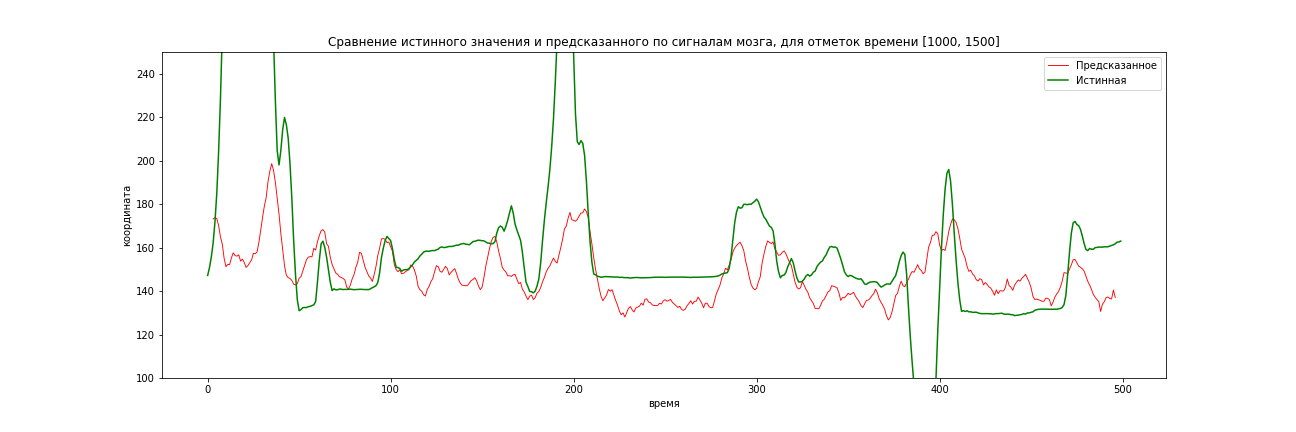
\includegraphics[scale=0.34]{images/1.png}
\end{figure}
\begin{figure}[H]
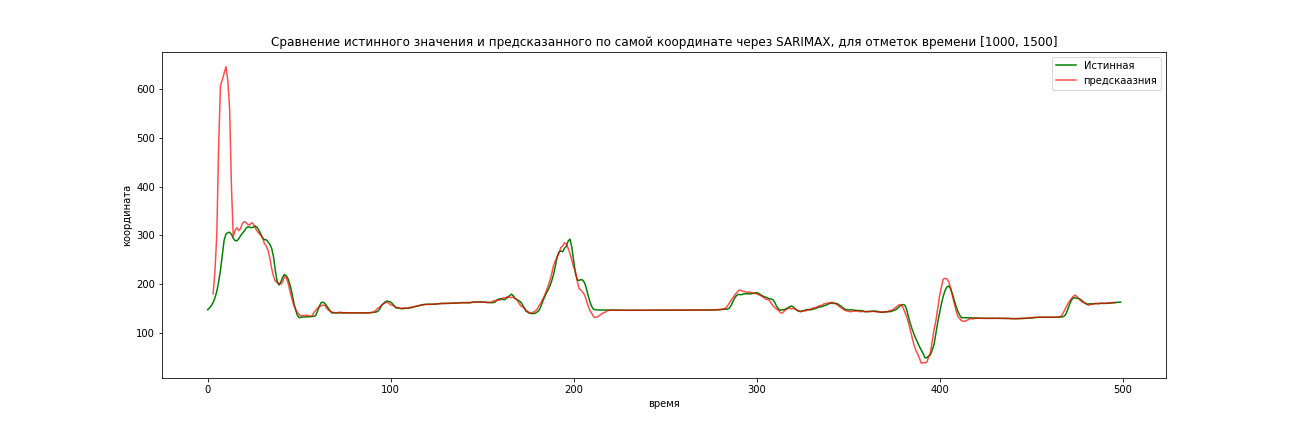
\includegraphics[scale=0.34]{images/2.png}
\end{figure}
\begin{figure}[H]
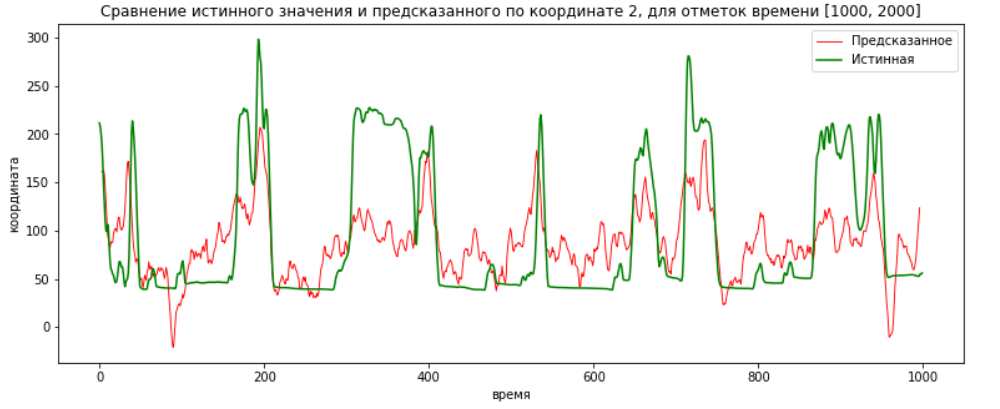
\includegraphics[scale=0.34]{images/3.png}
\end{figure}
\begin{figure}[H]
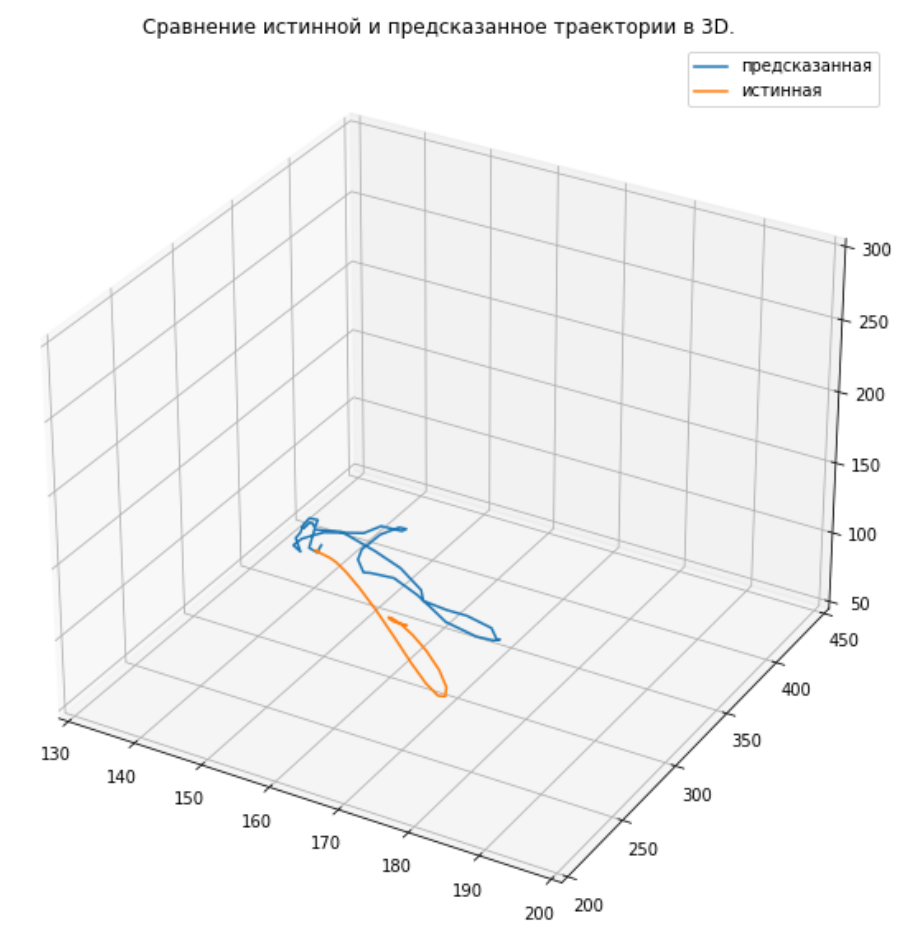
\includegraphics[scale=0.34]{images/4.png}
\end{figure}
Блендинг SARIMAX и PLS.
\begin{figure}[H]
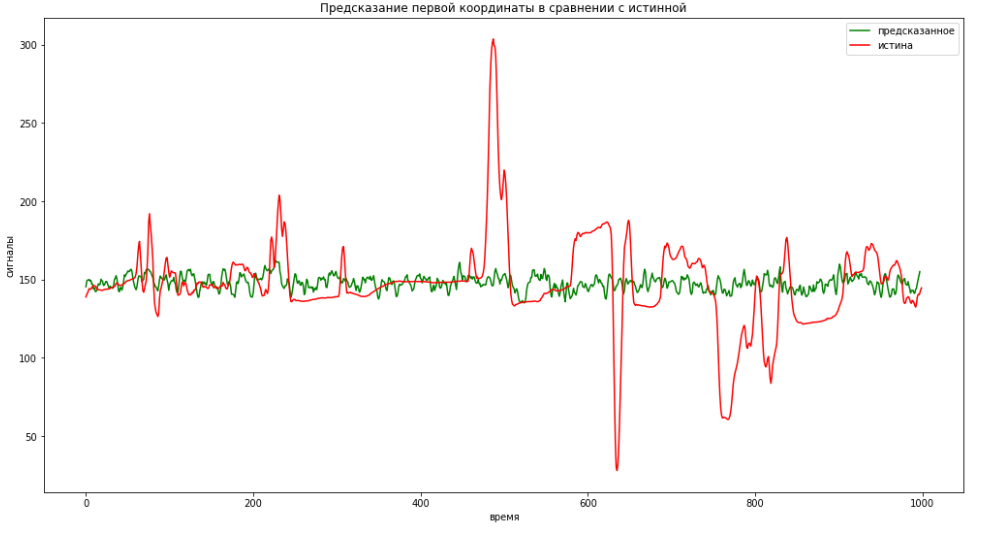
\includegraphics[scale=0.34]{images/5.png}
\end{figure}

Блендинг AR и PLS.
\begin{figure}[H]
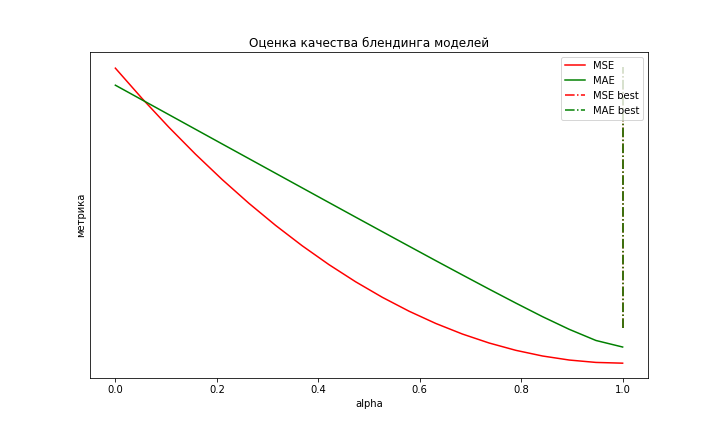
\includegraphics[scale=0.34]{images/6.png}
\end{figure}



\section{Сравнение моделей, анализ ошибок}
Рассматривается прогнозирование временного ряда координаты кисти, по прошлым точкам траектрии. Предлагается сравнить пять модели --- $PLS$ в чистом виде, $SARIMAX$ в чистом виде и их микс. А так же $AR$ в чистом виде и его блендинг с $PLS$. Сравнение происходит по метрикам $MSE, MAE$.
\begin{figure}[H]
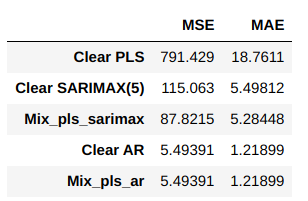
\includegraphics[scale=1]{images/7.png}
\end{figure}
Как видно, микс моделей SARIMAX и PLS дает лучший результат, чем каждая из них поотдельности. Но модель AR сама по себе настолько хороша, что даже блендинг с PLS не улучшает предсказание, а только портит. Можно сделать вывод, что простая AR лучшая модель.
\section{Заключение}



\nocite{*}
\bibliographystyle{plain}
\bibliography{references}



\end{document}
